\documentclass[a4paper,10pt]{scrartcl}
\usepackage[backend=biber,bibencoding=utf-8]{biblatex}

\usepackage{praeambel}

%%% Eigene Daten: Beginn
\title{Entwicklungsarbeit}
\newcommand\authorA{Sebastian Schramm}
\newcommand\matrikelnrA{-}
\newcommand\modul{Programmieren 1}
\newcommand\pruefer{-}
\date{\today}
%%% Eigene Daten: Ende

\begin{document}
\selectlanguage{ngerman}
\begin{titlepage}
  \pagestyle{empty}
  \centering

  \vspace*{0.5cm}
  \begin{otherlanguage*}{ngerman}
    \begin{sffamily} {
        \Large
        Hochschule -\\[1em]
        Fakultät IV -- Technische Informatik\\[0.1em]
        Modul: \modul\\[0.1em]
        Professor: \pruefer\\[0.1em]
      }
    \end{sffamily}
  \end{otherlanguage*}

  \vspace*{3cm}

  \begin{sffamily}
    \huge \bfseries
    \makeatletter
    \@title
    \makeatother
    \\
  \end{sffamily}

  \vspace*{1cm}

  \begin{otherlanguage*}{ngerman}
    
    \vspace*{3cm}
    
    von\\[0.75em]
    {
      \large
      \textbf{\authorA}\quad Matrikel-Nr. \matrikelnrA\\
      %\textbf{\authorB}\quad Matrikel-Nr. \matrikelnrB

      \vspace*{2cm}
      \makeatletter
      \@date
      \makeatother
    }
    \vfill
  \end{otherlanguage*}
\end{titlepage}

\tableofcontents

\newpage

%%% Protokoll: Beginn

% generated by Plantuml 1.2018.13      
\definecolor{plantucolor0000}{RGB}{0,0,0}
\definecolor{plantucolor0001}{RGB}{254,254,206}
\definecolor{plantucolor0002}{RGB}{168,0,54}
\begin{tikzpicture}[yscale=-1
	,pstyle0/.style={fill=black,line width=1.0pt}
	,pstyle3/.style={color=plantucolor0002,line width=1.5pt}
	,pstyle4/.style={color=plantucolor0002,fill=plantucolor0002,line width=1.0pt}
	]
	\draw[pstyle0] (101.3856pt,20pt) ellipse (10pt and 10pt);
	\draw[color=plantucolor0002,fill=plantucolor0001,line width=1.5pt] (10pt,66.9844pt) arc (180:270:16.9844pt) -- (26.9844pt,50pt) -- (175.7868pt,50pt) arc (270:360:16.9844pt) -- (192.7712pt,66.9844pt) -- (192.7712pt,66.9844pt) arc (0:90:16.9844pt) -- (175.7868pt,83.9688pt) -- (26.9844pt,83.9688pt) arc (90:180:16.9844pt) -- (10pt,66.9844pt) -- cycle;
	\node at (50pt,60pt)[below right,color=black]{print Dear Prudence};
	\draw[color=black,line width=1.0pt] (101.3856pt,113.9688pt) ellipse (10pt and 10pt);
	\draw[pstyle0] (101.8856pt,114.4688pt) ellipse (6pt and 6pt);
	\draw[pstyle3] (101.3856pt,30pt) -- (101.3856pt,50pt);
	\draw[pstyle4] (97.3856pt,40pt) -- (101.3856pt,50pt) -- (105.3856pt,40pt) -- (101.3856pt,44pt) -- cycle;
	\draw[pstyle3] (101.3856pt,83.9688pt) -- (101.3856pt,103.9688pt);
	\draw[pstyle4] (97.3856pt,93.9688pt) -- (101.3856pt,103.9688pt) -- (105.3856pt,93.9688pt) -- (101.3856pt,97.9688pt) -- cycle;
\end{tikzpicture}

\section{Kapitel 3}
\subsection{Teilaufgabe 1}
\subsubsection{Aufgabenstellung}
In der ersten Teilaufgabe sollten wir uns mit der Typkonvertierung befassen. Dafür schreiben wir
ein kleines Programm, welches die primitiven Datentypen erweiternd und einschränkend
Konvertiert.

\subsubsection{Anforderungsdefinition}
\begin{enumerate}
	\item Zu jedem Primitiven Datentypen eine erweiternde und einschränkende Konvertierung
	durchführen.
\end{enumerate}

\subsubsection{Entwurf}
Für die Aufgabe habe ich mich entschieden für jeden Primitive Datentyp einen Methode zu entwerfen, in
der letztendlich die Konvertierung für den entsprechenden Datentyp stattfinden wird.
\begin{center}
	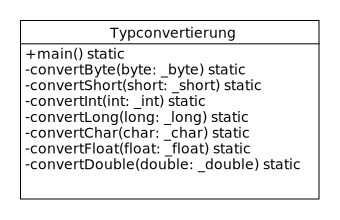
\includegraphics[width=0.6\textwidth]{uml/uml_c3_p1.pdf}
\end{center}

\subsubsection{Quelltext}
\paragraph{Typkonvertierungen.java}\
\lstinputlisting[language = Java , frame = trBL , escapeinside={(*@}{@*)}]{../chapter_03/src/main/java/chapter_03/Typkonvertierungen.java}

\subsubsection{Testdokumentation}
Nach den Aufruf des Programms, sollten alle Typkonvertierungen auf der Konsole ausgegeben
werden. Dies ist auch geschehen.

\subsubsection{Benutzungshinweise}
Keine Besonderen Benutzungshinweise.
Man navigiere zu dem Ordner von sich die Compilierte Datei mit dem Namen "Typkonvertierungen.class"
\space befindet und führt anschlie\ss end java Typkonvertierungen aus.

\subsubsection{Anwendungsbeispiel}
Nach dem man das Programm gestartet hat (aufgrund der Formatierung, werden einige Zeichen bei Char nicht dargestellt), sollte folgende Ausgabe erscheinen:

\begin{lstlisting}[frame = trBL , escapeinside={(*@}{@*)}]
[sebastian@laptop bin]$ java Typkonvertierungen
---------------------
Byte erweiternd
Byte   -128
Short  -128
Int    -128
Long   -128
Float  -128.0
Double -128.0

Char   タ
---------------------
Short einschränkend
Short  34
Byte   34
Short erweiternd
Short  34
Int    34
Long   34
Float  34.0
Double 34.0

Char   "
---------------------
Int einschränkend
Int    98987
Short  -32085
Byte   -85
Int erweiternd
Int    98987
Long   98987
Float  98987.0
Double 98987.0

Char   芫
---------------------
Long einschränkend
Long   987987987
Int    987987987
Short  -32749
Byte   19
Long erweiternd
Long   987987987
Float  9.8798797E8
Double 9.87987987E8

Char   耓
---------------------
Char einschränkend
Char   a
Long   97
Int    97
Short  97
Byte   97
Char erweiternd
Char   a
Long   97
Float  97.0
Double 97.0
---------------------
Float einschränkend
Float  15.0
Long   15
Int    15
Short  15
Byte   15
Float erweiternd
Float  15.0
Double 15.0

Char   
---------------------
Double einschränkend
Double 1.7976931348623157E308
Float  Infinity
Long   9223372036854775807
Int    2147483647
Short  -1
Byte   -1

Char   ￿
---------------------
[sebastian@laptop bin]$ 
\end{lstlisting}

% generated by Plantuml 1.2018.13      
\definecolor{plantucolor0000}{RGB}{0,0,0}
\definecolor{plantucolor0001}{RGB}{254,254,206}
\definecolor{plantucolor0002}{RGB}{168,0,54}
\begin{tikzpicture}[yscale=-1
,pstyle0/.style={fill=black,line width=1.0pt}
,pstyle1/.style={color=plantucolor0002,fill=plantucolor0001,line width=1.5pt}
,pstyle3/.style={color=plantucolor0002,line width=1.5pt}
,pstyle4/.style={color=plantucolor0002,fill=plantucolor0002,line width=1.0pt}
]
\draw[pstyle0] (99.5412pt,20pt) ellipse (10pt and 10pt);
\draw[pstyle1] (18.5775pt,66.9844pt) arc (180:270:16.9844pt) -- (35.5619pt,50pt) -- (163.5204pt,50pt) arc (270:360:16.9844pt) -- (180.5048pt,66.9844pt) -- (180.5048pt,66.9844pt) arc (0:90:16.9844pt) -- (163.5204pt,83.9688pt) -- (35.5619pt,83.9688pt) arc (90:180:16.9844pt) -- (18.5775pt,66.9844pt) -- cycle;
\node at (50pt,60pt)[below right,color=black]{print Byte min max};
\draw[pstyle1] (15.1634pt,120.9531pt) arc (180:270:16.9844pt) -- (32.1478pt,103.9688pt) -- (166.9346pt,103.9688pt) arc (270:360:16.9844pt) -- (183.919pt,120.9531pt) -- (183.919pt,120.9531pt) arc (0:90:16.9844pt) -- (166.9346pt,137.9375pt) -- (32.1478pt,137.9375pt) arc (90:180:16.9844pt) -- (15.1634pt,120.9531pt) -- cycle;
\node at (50pt,113.9688pt)[below right,color=black]{print Short min max};
\draw[pstyle1] (24.4139pt,174.9219pt) arc (180:270:16.9844pt) -- (41.3983pt,157.9375pt) -- (157.6841pt,157.9375pt) arc (270:360:16.9844pt) -- (174.6684pt,174.9219pt) -- (174.6684pt,174.9219pt) arc (0:90:16.9844pt) -- (157.6841pt,191.9063pt) -- (41.3983pt,191.9063pt) arc (90:180:16.9844pt) -- (24.4139pt,174.9219pt) -- cycle;
\node at (50pt,167.9375pt)[below right,color=black]{print Int min max};
\draw[pstyle1] (16.8831pt,228.8906pt) arc (180:270:16.9844pt) -- (33.8675pt,211.9063pt) -- (165.2149pt,211.9063pt) arc (270:360:16.9844pt) -- (182.1992pt,228.8906pt) -- (182.1992pt,228.8906pt) arc (0:90:16.9844pt) -- (165.2149pt,245.875pt) -- (33.8675pt,245.875pt) arc (90:180:16.9844pt) -- (16.8831pt,228.8906pt) -- cycle;
\node at (50pt,221.9063pt)[below right,color=black]{print Long min max};
\draw[pstyle1] (16.8794pt,282.8594pt) arc (180:270:16.9844pt) -- (33.8638pt,265.875pt) -- (165.2186pt,265.875pt) arc (270:360:16.9844pt) -- (182.203pt,282.8594pt) -- (182.203pt,282.8594pt) arc (0:90:16.9844pt) -- (165.2186pt,299.8438pt) -- (33.8638pt,299.8438pt) arc (90:180:16.9844pt) -- (16.8794pt,282.8594pt) -- cycle;
\node at (50pt,275.875pt)[below right,color=black]{print Char min max};
\draw[pstyle1] (10pt,336.8281pt) arc (180:270:16.9844pt) -- (26.9844pt,319.8438pt) -- (172.098pt,319.8438pt) arc (270:360:16.9844pt) -- (189.0824pt,336.8281pt) -- (189.0824pt,336.8281pt) arc (0:90:16.9844pt) -- (172.098pt,353.8125pt) -- (26.9844pt,353.8125pt) arc (90:180:16.9844pt) -- (10pt,336.8281pt) -- cycle;
\node at (50pt,329.8438pt)[below right,color=black]{print Double min max};
\draw[pstyle1] (16.3831pt,390.7969pt) arc (180:270:16.9844pt) -- (33.3675pt,373.8125pt) -- (165.7149pt,373.8125pt) arc (270:360:16.9844pt) -- (182.6992pt,390.7969pt) -- (182.6992pt,390.7969pt) arc (0:90:16.9844pt) -- (165.7149pt,407.7813pt) -- (33.3675pt,407.7813pt) arc (90:180:16.9844pt) -- (16.3831pt,390.7969pt) -- cycle;
\node at (50pt,383.8125pt)[below right,color=black]{print Float min max};
\draw[color=black,line width=1.0pt] (99.5412pt,437.7813pt) ellipse (10pt and 10pt);
\draw[pstyle0] (100.0412pt,438.2813pt) ellipse (6pt and 6pt);
\draw[pstyle3] (99.5412pt,30pt) -- (99.5412pt,50pt);
\draw[pstyle4] (95.5412pt,40pt) -- (99.5412pt,50pt) -- (103.5412pt,40pt) -- (99.5412pt,44pt) -- cycle;
\draw[pstyle3] (99.5412pt,83.9688pt) -- (99.5412pt,103.9688pt);
\draw[pstyle4] (95.5412pt,93.9688pt) -- (99.5412pt,103.9688pt) -- (103.5412pt,93.9688pt) -- (99.5412pt,97.9688pt) -- cycle;
\draw[pstyle3] (99.5412pt,137.9375pt) -- (99.5412pt,157.9375pt);
\draw[pstyle4] (95.5412pt,147.9375pt) -- (99.5412pt,157.9375pt) -- (103.5412pt,147.9375pt) -- (99.5412pt,151.9375pt) -- cycle;
\draw[pstyle3] (99.5412pt,191.9063pt) -- (99.5412pt,211.9063pt);
\draw[pstyle4] (95.5412pt,201.9063pt) -- (99.5412pt,211.9063pt) -- (103.5412pt,201.9063pt) -- (99.5412pt,205.9063pt) -- cycle;
\draw[pstyle3] (99.5412pt,245.875pt) -- (99.5412pt,265.875pt);
\draw[pstyle4] (95.5412pt,255.875pt) -- (99.5412pt,265.875pt) -- (103.5412pt,255.875pt) -- (99.5412pt,259.875pt) -- cycle;
\draw[pstyle3] (99.5412pt,299.8438pt) -- (99.5412pt,319.8438pt);
\draw[pstyle4] (95.5412pt,309.8438pt) -- (99.5412pt,319.8438pt) -- (103.5412pt,309.8438pt) -- (99.5412pt,313.8438pt) -- cycle;
\draw[pstyle3] (99.5412pt,353.8125pt) -- (99.5412pt,373.8125pt);
\draw[pstyle4] (95.5412pt,363.8125pt) -- (99.5412pt,373.8125pt) -- (103.5412pt,363.8125pt) -- (99.5412pt,367.8125pt) -- cycle;
\draw[pstyle3] (99.5412pt,407.7813pt) -- (99.5412pt,427.7813pt);
\draw[pstyle4] (95.5412pt,417.7813pt) -- (99.5412pt,427.7813pt) -- (103.5412pt,417.7813pt) -- (99.5412pt,421.7813pt) -- cycle;
\end{tikzpicture}


\printbibliography

%%% Protokoll: Ende
\end{document}